% (c) 2017 Daniele Zambelli - daniele.zambelli@gmail.com
% (c) 2012 Dimitrios Vrettos - d.vrettos@gmail.com
% 
% Tutti i grafici per il capitolo interi.tex
% 

\newcommand{\everest}{
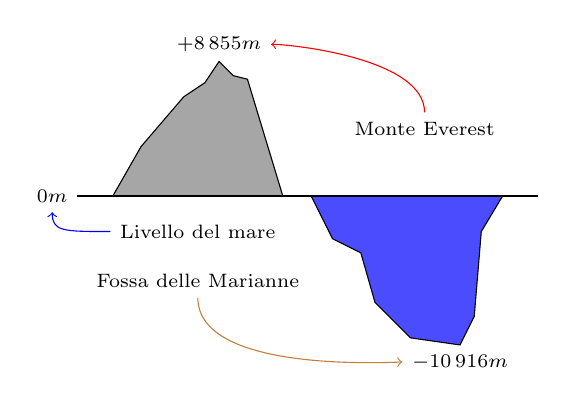
\begin{tikzpicture}[scale=.9]
  % Disegna Everest
  \filldraw[fill=gray!70, draw=black] (0,0)-- (4mm,7mm)-- 
(10mm,14mm)--(13mm,16mm)-- (15mm,19mm)--(17mm,17mm)--%
	    (19mm,16.5mm)--(24mm,0);
  % Disegna Fossa delle Marianne
  \filldraw[fill=blue!70, 
draw=black](28mm,0)--(31mm,-6mm)--(35mm,-8mm)--(37mm,-15mm)--(42mm,-20mm)-- 
(49mm,-21mm)--%
	    (51mm, -17mm)--(52mm, -5mm)--(55mm,0);
  % Disegna il livello del mare 
  \draw[thick] (-5mm,0) -- (60mm,0);

  \begin{scope}[font=\scriptsize]
    % Posiziona altezze
    \node[left] (0)at (-5mm,0) {$0\unit{m}$};
    \node [above](everest) at (15mm,19mm) {$+8\,855\unit{m}$};
    \node [below](marianne) at (49mm,-21mm) {$-10\,916\unit{m}$};
    % Posiziona etichette
    \node (testo1) at (44mm,9.5mm) {Monte Everest};
    \node (testo2) at (12mm,-5mm) {Livello  del mare};
    \node (testo3) at (12mm,-12mm) {Fossa delle Marianne};
  \end{scope}
  % Disegna frecce
  \draw[<-,red ] (everest) .. controls +(right:10mm) and +(up:10mm) .. 
node[]{} (testo1);
  \draw[<-, blue](0)..controls +(down:5mm) and +(left:19mm)..node[]{} 
(testo2);
  \draw[<-, brown](marianne)..controls +(left:10mm) and +(down:13mm)..node[]{} 
(testo3);

\end{tikzpicture}
}

\newcommand{\rettainteri}{
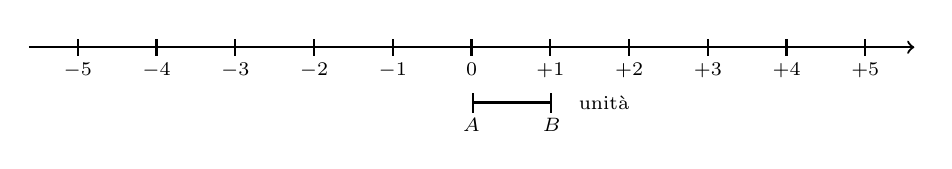
\begin{tikzpicture}
\begin{scope}[thick,font=\scriptsize]
  \draw[->] (-160pt,0)  - -  (160pt,0) node[above]{$\Z$};	
    \foreach \n in {-5,-4,...,0}{%
      \draw (\n,-3pt) -- (\n,3pt)   node [below=5pt] {$\n$};		
    }

    \foreach \m in {1,2,...,5}{%
      \draw (\m,-3pt) -- (\m,3pt) node [below=5pt]{+$\m$};
    }
  
    \draw[|-|]node [below=22pt]{$A$}(0,-20pt)--(29pt,-20pt) 
node[below=2pt]{$B$};

    \node [right] at (+35pt,-20pt) {unit\`a};
\end{scope}

\end{tikzpicture}
}

\newcommand{\esec}{
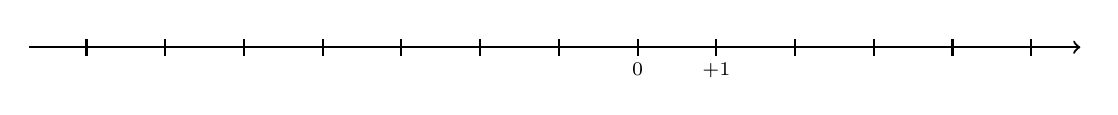
\begin{tikzpicture}

\begin{scope}[thick,font=\scriptsize]
  \draw[->] (-220pt,0)  - -  (160pt,0) node[above]{$\Z$};	
    \foreach \n in {-7,-6,...,-1}{%
      \draw (\n,-3pt) -- (\n,3pt)   node [below=5pt] {};		
    }

    \foreach \m in {2,3,...,5}{%
      \draw (\m,-3pt) -- (\m,3pt) node [below=5pt]{};
    }

    \foreach \x in {1}{%
      \draw (\x,-3pt) -- (\x,3pt) node [below=5pt]{+$\x$};
    }
    
    \foreach \y in {0}{%
      \draw (\y,-3pt) -- (\y,3pt) node [below=5pt]{$\y$};
    }
\end{scope}
\end{tikzpicture}
}

\newcommand{\sommaa}{
\begin{tikzpicture}[decoration={markings,mark=between positions 0.7 and .9 
step 30pt with {\arrow{stealth}}}]
  \begin{scope}[thick,font=\scriptsize]
   \draw[->] (-160pt,0)  - -  (110pt,0) node[above]{$\Z$};
    \foreach \c in {-3,-2,...,1}{%
     \draw[dotted, color=RedOrange,postaction={decorate}](\c,5pt)--(\c,5pt) 
arc (180:0:0.5 and 0.5);}
    \foreach \n in {-5,-4,...,0}{%	
     \draw (\n,-3pt) -- (\n,3pt)   node [below=5pt] {$\n$};}
    \foreach \m in {1,2,3}{%	
     \draw (\m,-3pt) -- (\m,3pt)   node [below=5pt] {$+\m$};}

  \end{scope}
 \end{tikzpicture}
}

\newcommand{\sommab}{
 \begin{tikzpicture}[decoration={markings,mark=between positions .3 and .5 
step 30pt with {\arrowreversed{stealth}}}]
  \begin{scope}[thick,font=\scriptsize]
   \draw[->] (-160pt,0)  - -  (110pt,0) node[above]{$\Z$};
    \foreach \c in {-4,-3,-2}{%
     \draw[dotted, 
color=CornflowerBlue,postaction={decorate}](\c,5pt)--(\c,5pt) arc (180:0:0.5 
and 0.5);}
    \foreach \n in {-5,-4,...,0}{%	
     \draw (\n,-3pt) -- (\n,3pt)   node [below=5pt] {$\n$};}
    \foreach \m in {1,2,3}{%	
     \draw (\m,-3pt) -- (\m,3pt)   node [below=5pt] {$+\m$};}

  \end{scope}
 \end{tikzpicture}
}

\newcommand{\sottrazione}{
\begin{tikzpicture}
% % \begin{scope}[font=\scriptsize]
% \matrix [matrix of math nodes,column sep={10mm,between origins}] at (0,0)
% {
% \node{(+2)};& \node[circle, draw=red](-){-}; & \node[draw=blue,circle] 
% (3pos){(+3)} ;%
% & \node{=};& \node{(+2)};& \node[circle, draw=red](+){+};& 
% \node[draw=blue,circle](3neg){(-3)};\\
% };


% \node (testo1) at (0, -15mm) {Cambio il numero $+3$ con il suo opposto $-3$};
% \node (testo2) at (0,15mm) {Cambio la sottrazione in addizione};
% % \end{scope}
% 
%  \draw[->,red ] (testo2) .. controls +(down:5mm) and +(up:10mm) .. (-) ;
%  \draw[->,red ] (testo2) .. controls +(down:5mm) and +(up:10mm) .. (+) ;
% 
%  \draw[->,blue ] (testo1) .. controls +(up:10mm) and +(down:10mm) .. (3neg) ;
%  \draw[->,blue ] (testo1) .. controls +(up:10mm) and +(down:10mm) .. (3pos) ;

\end{tikzpicture}
}

\newcommand{\moltsegni}{
\begin{tikzpicture}[font=\Huge]

% \matrix (segni) [matrix of nodes]{%
%  $\cdot$& $+$ & $-$\\
%  $+$& $+$ &$-$\\
%  $-$& $-$ &$+$\\
% };
% 
%   \begin{scope}[thin, blue]
%     \draw (segni-2-1.north west)--(segni-2-3.north east);
%     \draw (segni-1-2.north west)--(segni-3-2.south west);
%   \end{scope}
\end{tikzpicture}
}

